\begin{appendices}

	\section{Alloy model}
		\subsection{Source code}
		\lstinputlisting[language=alloy]{alloy/alloy2.0version.als}
		\begin{figure}[h!]
			\centering
			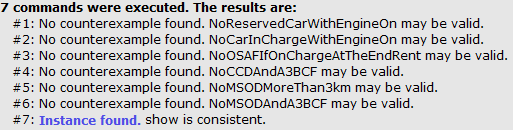
\includegraphics[]{alloy/AlloyResult.png}
			\caption{
				\label{fig:alloyExecutionResult} 
				Alloy execution result
			}
		\end{figure}
		\clearpage
		\subsection{Generated worlds}
			Note that in \autoref{fig:alloyWorld1} LoggedUser3 has been banned \emph{after} completing RentMade0.
			\begin{figure}[h!]
			\centering
			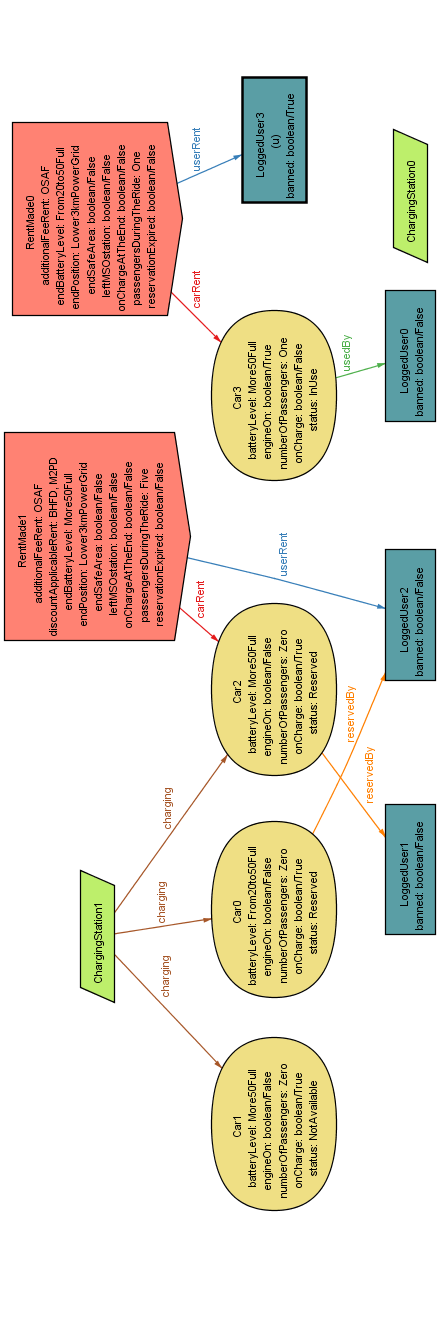
\includegraphics[scale=0.39]{alloy/AlloyWorld2.png}
			\caption{
				\label{fig:alloyWorld1} 
				First alloy generated world
			}
		\end{figure}
		\clearpage
		Note that in \autoref{fig:alloyWorld2} RentMade1 is actually a reservation expired of Car3 made by LoggedUser2. He now has reserved Car1.
		\begin{figure}[h!]
		\centering
		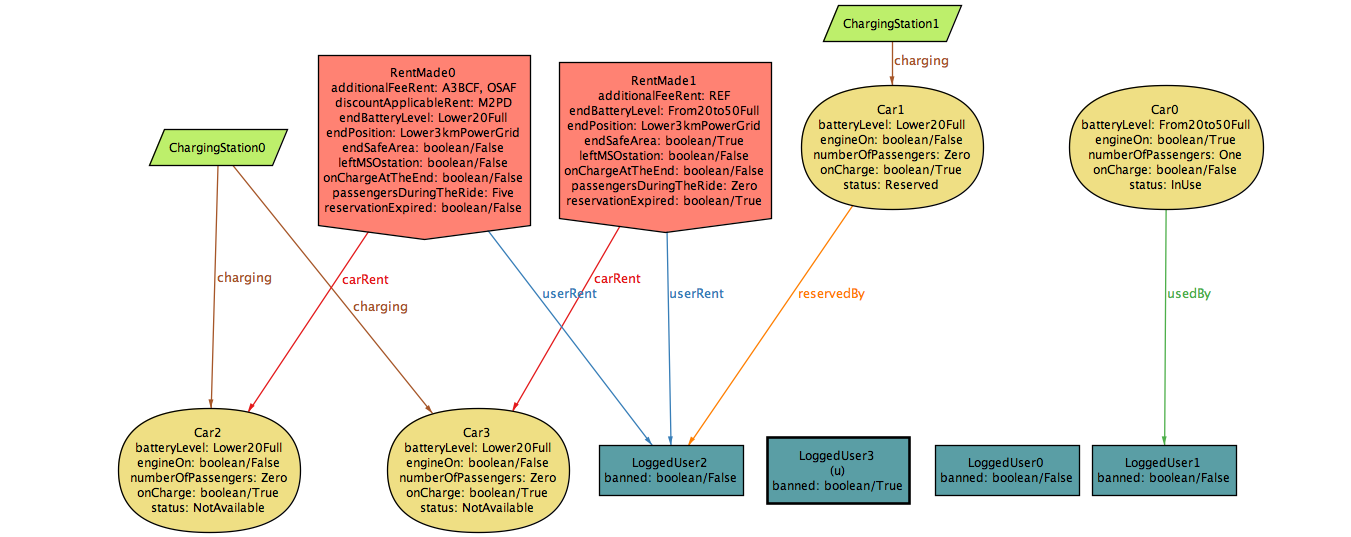
\includegraphics[scale=0.39]{alloy/AlloyWorld1.png}
		\caption{
			\label{fig:alloyWorld2} 
			Second alloy generated world
		}
		\end{figure}
		\clearpage
	\section{Software and tools used}
	For the development of this document we used
	\begin{itemize}
		\item \LaTeX{} as document preparation system
		\item Git \& \href{http://github.com}{GitHub} as version control system
		\item \href{http://draw.io}{Draw.io} for graphs
		\item StarUML for diagrams
		\item Alloy as model analyzer
	\end{itemize}
	
	\section{Hours of work}
	This is the time spent for redact this document
	\begin{itemize}
		\item Davide Piantella: $\sim$ 48 hours
		\item Mario Scrocca: $\sim$ 48 hours
		\item Moreno R. Vendra: $\sim$ 45 hours
	\end{itemize}
\end{appendices}
\clearpage
\begin{thebibliography}{9}
\bibitem{RE}B. Nuseibeh, S. Easterbrook, \emph{Requirements Engineering: A Roadmap}, 2000
\bibitem{Zave}P. Zave, \emph{Classification of Research Efforts in Requirements
Engineering}, ACM Computing Surveys, 1997
\bibitem{IeeeRasd}IEEE Std 830:1993, \emph{IEEE Recommended Practice for Software Requirements Specifications}, 1993
\bibitem{WorldMachine}M. Jackson, \emph{The World and the Machine}, 1995
\bibitem{TextualAnalysis}R. J. Abbot, \emph{Textual (noun-verb) analysis},1983
\end{thebibliography}